\documentclass[a4paper,12pt]{article}
\usepackage[utf8]{inputenc}
\usepackage[T1]{fontenc}
\usepackage[polish]{babel}
\usepackage{polski}
\usepackage{geometry}
\geometry{margin=2cm}
\usepackage[colorlinks=true, linkcolor=black]{hyperref}
\usepackage{booktabs}
\usepackage{longtable}
\usepackage{graphicx}
\usepackage{float}
\usepackage{caption}
\usepackage{amssymb}
\usepackage{amsmath}
\usepackage{pdflscape}
\usepackage{tabularx}

\title{Systemy Wbudowane 2026 \\ Projekt \\ Sterownik windy}
\author{Jan Brzoska \\ Michał Loński}
\date{}

\begin{document}
\maketitle
\renewcommand{\contentsname}{Spis treści}
\tableofcontents
\pagebreak
\renewcommand{\arraystretch}{1.5}
\section{Opis systemu}

\subsection{Wprowadzenie}
Sterownik windy jest systemem odpowiedzialnym za zarządzanie pionowym ruchem kabiny windy w budynku wielopiętrowym.
\subsection{Funkcjonalności}
Główną funkcjonalnością systemu jest transport pasażerów pomiędzy piętrami budynku.
\subsubsection{Funkcjonalności podstawowe}
\begin{itemize}
    \item przyjmowanie i kolejkowanie zgłoszeń (wezwanie windy)
    \item obsługa wyboru pięter w windzie
    \item sterowanie ruchem windy (ruch w górę, dół oraz zatrzymanie się)
    \item otwieranie i zamykanie drzwi windy
\end{itemize}
\subsubsection{Funkcjonalności wtórne}
\begin{itemize}
    \item optymalizacja kolejności przystanków
    \item obsługa wielu wind
    \item wzywanie serwisu/pomocy
    \item wykrywanie przeciążenia i reagowanie na nie
    \item tryby specjalne (awaryjny, serwisowy)
    \item ograniczony dostęp do poszczególnych pięter, wymagający uprawnień (np. karty pracownika)
    \item monitorowanie stanu systemu
    \item wyświetlanie informacji o piętrze, emitowanie komunikatów głosowych
\end{itemize}
\subsection{Sposób działania}
System przetwarza sygnały wejściowe i wysyła odpowiednie sygnały wyjściowe.
\bigskip
\\
\textbf{Wejścia do systemu:}
\begin{itemize}
    \item przyciski na piętrach (góra/dół)
    \item przyciski w kabinie windy (wybór piętra, otwarcie/zamknięcie drzwi, wezwanie pomocy)
    \item czujniki położenia kabiny
    \item czujniki drzwi
    \item czujniki obciążenia
    \item czytnik kart lub innej formy weryfikacji uprawnień
\end{itemize}
\bigskip
\textbf{Wyjścia systemu:}
\begin{itemize}
    \item sterowanie silnikiem (kierunek i prędkość)
    \item sterowanie drzwiami
    \item sygnalizacja (wyświetlacze, dźwięki)
    \item oświetlenie windy
\end{itemize}
\bigskip
Sterownik analizuje aktualny stan systemu i wyznacza optymalne decyzje o kierunku ruchu oraz kolejności obsługi zgłoszeń.
Ruch windy zależny jest od trybu pracy windy oraz domknięcia drzwi.
Optymalność polega na minimalizacji liczby zatrzymań windy oraz minimalizacja czasu oczekiwania pasażerów na windę.
\subsection{Środowisko pracy}
System działa w budynkach wielopiętrowych, takich jak:
\begin{itemize}
    \item budynki mieszkalne
    \item biurowce
    \item centra handlowe
    \item szpitale
\end{itemize}
Ze względu na swoją rolę, system posiada następujące wymagania:
\begin{itemize}
    \item przystosowanie do pracy w szybie windy (wąskie zakresy tolerancji temperatur, zakłócenia elektromagnetyczne)
    \item wysoki poziom bezpieczeństwa (zatrzymanie awaryjne, połączenie z systemem oddymiania)
    \item możliwość pracy w trybie awaryjnym przy zaniku zasilania głównego
    \item niezawodność, odporność na awarie
    \item zgodność z normami technicznymi
\end{itemize}
\subsection{Użytkownicy systemu}
System jest używany przez różne grupy użytkowników:
\begin{itemize}
    \item pasażerowie - korzystający z windy do przemieszczania się lub do transportu towarów
    \item serwis techniczny - odpowiedzialny za konserwację i diagnostykę
    \item służby ratunkowe - korzystające z trybów specjalnych (np. pożarowych)
\end{itemize}
\pagebreak
\section{Przypadki użycia}

\begin{table}[h]
\centering
\begin{tabular}{|p{0.3\textwidth}|p{0.35\textwidth}|p{0.25\textwidth}|}
\hline
\textbf{Use Case Name:} Wezwanie windy & \textbf{Use Case Number:} 1 & \textbf{Priority:} Medium \\ \hline
\textbf{Primary Actor:} Pasażer & \multicolumn{2}{l|}{\textbf{Use Case Type:} Essential} \\ \hline
\multicolumn{3}{|p{0.9\textwidth}|}{\textbf{Stakeholders and Interests:} \newline
\textbf{Pasażer:} wzywa windę na swoje piętro. \newline
\textbf{System:} rejestruje zgłoszenie i uwzględnia je w planowaniu.} \\ \hline
\multicolumn{3}{|p{0.9\textwidth}|}{\textbf{Brief description:} Proces zgłoszenia wezwania windy z poziomu piętra za pomocą przycisku kierunkowego.} \\ \hline
\textbf{Trigger:} Naciśnięcie przycisku (góra/dół) & \multicolumn{2}{l|}{\textbf{Type:} External} \\ \hline
\multicolumn{3}{|p{0.9\textwidth}|}{\textbf{Relationships:} \newline
\textbf{Include:} Zarządzanie kolejką zgłoszeń } \\ \hline
\multicolumn{3}{|p{0.9\textwidth}|}{\textbf{Normal Flow of Events:} \newline
1. Pasażer naciska przycisk kierunku jazdy (góra/dół). \newline
2. System rejestruje zgłoszenie wraz z kierunkiem. \newline
3. System analizuje pozycję wszystkich kabin i przydziela tę, która dotrze najszybciej. \newline
4. Zgłoszenie zostaje dodane do kolejki obsługi.} \\ \hline
\multicolumn{3}{|p{0.9\textwidth}|}{\textbf{Subflows:}} \\ \hline
\multicolumn{3}{|p{0.9\textwidth}|}{\textbf{Alternate/Exception Flows:} \newline
\textbf{Ex. 1:} System w trybie awaryjnym - zgłoszenie ignorowane. \newline
\textbf{Ex. 2:} Naciśnięcie obu przycisków kierunku - zgłoszenie ignorowane.} \\ \hline
\end{tabular}
\end{table}

\pagebreak

\begin{table}[h]
\centering
\begin{tabular}{|p{0.3\textwidth}|p{0.35\textwidth}|p{0.25\textwidth}|}
\hline
\textbf{Use Case Name:} Wybór piętra w kabinie & \textbf{Use Case Number:} 2 & \textbf{Priority:} Medium \\ \hline
\textbf{Primary Actor:} Pasażer & \multicolumn{2}{l|}{\textbf{Use Case Type:} Detail, essential} \\ \hline
\multicolumn{3}{|p{0.9\textwidth}|}{\textbf{Stakeholders and Interests:} \newline
\textbf{Pasażer:} wybiera docelowe piętro. \newline
\textbf{System:} uwzględnia wybór w planie jazdy.} \\ \hline
\multicolumn{3}{|p{0.9\textwidth}|}{\textbf{Brief description:} Wybór piętra docelowego wewnątrz kabiny windy.} \\ \hline
\textbf{Trigger:} Naciśnięcie przycisku w windzie & \multicolumn{2}{l|}{\textbf{Type:} External} \\ \hline
\multicolumn{3}{|p{0.9\textwidth}|}{\textbf{Relationships:} \newline
\textbf{Include:} Zarządzanie kolejką zgłoszeń} \\ \hline
\multicolumn{3}{|p{0.9\textwidth}|}{\textbf{Normal Flow of Events:} \newline
1. Pasażer naciska przycisk w kabinie: \newline
\hspace*{10pt} $\bullet$ jeśli naciśnięto przycisk otwarcia drzwi: przejdź do podprzepływu S1. \newline
\hspace*{10pt} $\bullet$ jeśli naciśnięto przycisk zamknięcia drzwi: przejdź do podprzepływu S2. \newline
\hspace*{10pt} $\bullet$ jeśli naciśnięto przycisk alarmowy i przytrzymano: przejdź do podprzepływu S3. \newline
\hspace*{10pt} $\bullet$ jeśli wybrano piętro: przejdź do podprzepływu S4. \newline
2. System rejestruje wybór i podświetla przycisk. \newline
3. System dodaje piętro do listy przystanków i aktualizuje plan jazdy windy. \newline
} \\ \hline
\multicolumn{3}{|p{0.9\textwidth}|}{\textbf{Subflows:} \newline
\textbf{S1:} System zamyka drzwi kabiny. \newline
\textbf{S2:} System otwiera drzwi kabiny. \newline
\textbf{S3:} System nawiązuje połączenie między pasażerem a ochroną. \newline
\textbf{S4:} 1. Jeśli wybrane piętro nie wymaga specjalnych uprawnień kontynuuj przepływ główny. \newline
             \hspace*{20pt} 2. Oczekuj na przyłożenie karty dostępu do czytnika. \newline
             \hspace*{20pt} 3. Powrót do przepływu głównego. \newline
} \\ \hline
\multicolumn{3}{|p{0.9\textwidth}|}{\textbf{Alternate/Exception Flows:} \newline
\textbf{Ex. 1:} Brak wymaganych uprawnień - sygnał dźwiękowy i zignorowanie wyboru.} \\ \hline
\end{tabular}
\end{table}

\pagebreak
\begin{table}[h]
\centering
\begin{tabular}{|p{0.3\textwidth}|p{0.35\textwidth}|p{0.25\textwidth}|}
\hline
\textbf{Use Case Name:} Realizacja przejazdu & \textbf{Use Case Number:} 3 & \textbf{Priority:} High \\ \hline
\textbf{Primary Actor:} System & \multicolumn{2}{l|}{\textbf{Use Case Type:} Detail, essential} \\ \hline

\multicolumn{3}{|p{0.9\textwidth}|}{\textbf{Stakeholders and Interests:} \newline
\textbf{Pasażer:} korzysta z kabiny windy. \newline
\textbf{System sterowania:} realizuje żądania z kolejki. \newline
\textbf{Sterownik napędu:} wykonuje ruch kabiny. \newline
\textbf{Czujniki:} dostarczają dane o pozycji kabiny i stanie drzwi.} \\ \hline

\multicolumn{3}{|p{0.9\textwidth}|}{\textbf{Brief description:} System realizuje przejazd kabiny windy do kolejnych celów znajdujących się w kolejce żądań.} \\ \hline

\textbf{Trigger:} Zmiana stanu kolejki żądań & \multicolumn{2}{l|}{\textbf{Type:} Internal} \\ \hline

\multicolumn{3}{|p{0.9\textwidth}|}{\textbf{Relationships:} \newline
\textbf{Include:} sterowanie ruchem, obsługa drzwi} \\ \hline

\multicolumn{3}{|p{0.9\textwidth}|}{\textbf{Normal Flow of Events:} \newline
1. System odczytuje stan kolejki żądań. \newline
\hspace*{10pt} $\bullet$ jeśli kolejka pusta: zakończ przepływ. \newline
\hspace*{10pt} $\bullet$ jeśli kolejka niepusta: kontynuuj główny przepływ. \newline
2. System wybiera pierwsze żądanie z kolejki według priorytetu i wyznacza docelowe piętro. \newline
3. System zamyka drzwi i rygluje je. \newline
4. System generuje polecenie ruchu kabiny do sterownika napędu. \newline
5. System realizuje ruch kabiny do wyznaczonego piętra monitorując czujniki pozycji. \newline
6. Po osiągnięciu piętra celowego system zatrzymuje kabinę, wyrównuje poziom do progu. \newline
7. System otwiera drzwi. \newline
8. System usuwa zrealizowane żądanie z kolejki. \newline
9. System powraca do kroku 1.} \\ \hline
\multicolumn{3}{|p{0.9\textwidth}|}{\textbf{Subflows:} } \\ \hline
\multicolumn{3}{|p{0.9\textwidth}|}{\textbf{Alternate/Exception Flows:} \newline
\textbf{Ex. 1:} Wykrycie przeszkody w drzwiach - wstrzymanie zamykania drzwi z próbą powtórzenia po interwale czasowym. \newline
\textbf{Ex. 2:} Tryb awaryjny - zignorowanie kolejki żądań, kierowanie się na wyznaczone odgórnie piętro. \newline
\textbf{Ex. 3:} Wezwanie serisowe - zignorowanie priorytetów.} \\ \hline

\end{tabular}
\end{table}
\pagebreak
\begin{table}[h]
\centering
\begin{tabular}{|p{0.3\textwidth}|p{0.35\textwidth}|p{0.25\textwidth}|}
\hline
\textbf{Use Case Name:} Konfiguracja parametrów & \textbf{Use Case Number:} 1 & \textbf{Priority:} High \\ \hline
\textbf{Primary Actor:} Serwisant, System & \multicolumn{2}{l|}{\textbf{Use Case Type:} Detail, essential} \\ \hline
\multicolumn{3}{|p{0.9\textwidth}|}{\textbf{Stakeholders and Interests:} \newline
\textbf{Serwisant:} dostosowuje pracę windy do specyfiki budynku (czas otwarcia drzwi, prędkość). \newline
\textbf{System:} odbiera parametry niezbędne do poprawnego wyliczania krzywej hamowania i logiki drzwi. \newline
\textbf{Baza danych:} przechowuje nastawy w pamięci nieulotnej.} \\ \hline
\multicolumn{3}{|p{0.9\textwidth}|}{\textbf{Brief description:} Ten UC opisuje proces wprowadzania nastaw serwisowych przez technika, takich jak czas podtrzymania otwartych drzwi, prędkość nominalna oraz piętro bazowe.} \\ \hline
\textbf{Trigger:} Serwisant (aktywacja przełącznika trybu) & \multicolumn{2}{l|}{\textbf{Type:} External} \\ \hline
\multicolumn{3}{|p{0.9\textwidth}|}{\textbf{Relationships:} \newline
\textbf{Association:} Baza danych (Pamięć konfiguracji) } \\ \hline
\multicolumn{3}{|p{0.9\textwidth}|}{\textbf{Normal Flow of Events:} \newline
1. Serwisant naciska jeden z przycisków „SET” na panelu sterowniczym (np. SET\_TIME, SET\_SPEED).  \newline
2. System wyświetla aktualną wartość na wyświetlaczu i umożliwia wprowadzenie nowej za pomocą klawiatury numerycznej. \newline
3. Po wprowadzeniu wartości, Serwisant naciska przycisk APPLY, aby zatwierdzić zmianę, lub RESET, aby porzucić edycję. \newline
\hspace*{10pt} $\bullet$ jeśli APPLY: przejdź do podprzepływu S1. \newline
\hspace*{10pt} $\bullet$ jeśli RESET: przejdź do podprzepływu S2. \newline
4. Serwisant wybiera kolejny parametr do ustawienia (SET), kończy pracę (DONE) lub resetuje sterownik. \newline
\hspace*{10pt} $\bullet$ jeśli SET – powrót do kroku. \newline
\hspace*{10pt} $\bullet$ jeśli DONE – przejdź do kroku. \newline
5. Nowe dane są przesyłane do pamięci nieulotnej sterownika. \newline
6. System wyświetla komunikat o poprawnym zapisaniu konfiguracji.} \\ \hline
\multicolumn{3}{|p{0.9\textwidth}|}{\textbf{Subflows:} \newline
\textbf{S1:} \newline
\hspace*{10pt} $\bullet$ Nowe dane są sprawdzane pod kątem dopuszczalnych zakresów (walidacja). \newline
\hspace*{10pt} $\bullet$ Jeśli poprawne, zostają tymczasowo zapisane w pamięci RAM; jeśli błędne, wyświetlany jest błąd zakresu. \newline
\textbf{S2:} \newline
\hspace*{10pt} $\bullet$ Nowe dane nie są zapisywane; system przywraca poprzedni stan i przechodzi do kroku 4.} \\ \hline
\multicolumn{3}{|p{0.9\textwidth}|}{\textbf{Alternate/Exception Flows:} \newline
\textbf{Ex. 1:} Jednoczesne naciśnięcie dwóch przycisków – sygnał dźwiękowy (beep) i ignorowanie wejścia. \newline
\textbf{Ex. 2:} Błąd zapisu do pamięci EEPROM – wyświetlenie ostrzeżenia o awarii modułu pamięci.} \\ \hline
\end{tabular}
\end{table}

\pagebreak

\begin{table}[h]
\centering
\begin{tabular}{|p{0.3\textwidth}|p{0.35\textwidth}|p{0.25\textwidth}|}
\hline
\textbf{Use Case Name:} Tryb awaryjny & \textbf{Use Case Number:} 5 & \textbf{Priority:} Critical \\ \hline
\textbf{Primary Actor:} System PPOŻ & \multicolumn{2}{l|}{\textbf{Use Case Type:} Essential} \\ \hline
\multicolumn{3}{|p{0.9\textwidth}|}{\textbf{Stakeholders and Interests:} \newline
\textbf{System PPOŻ:} przekazuje sygnał zagrożenia. \newline
\textbf{System windy:} zapewnia bezpieczeństwo pasażerów. \newline
\textbf{Pasażer:} powinien zostać ewakuowany.} \\ \hline
\multicolumn{3}{|p{0.9\textwidth}|}{\textbf{Brief description:} Reakcja windy na sygnał alarmowy.} \\ \hline
\textbf{Trigger:} Sygnał alarmowy z systemu PPOŻ lub innego systemu bezpieczeństwa & \multicolumn{2}{l|}{\textbf{Type:} External} \\ \hline
\multicolumn{3}{|p{0.9\textwidth}|}{\textbf{Relationships:} \newline
\textbf{Extend:} Wszystkie podstawowe use case’y} \\ \hline
\multicolumn{3}{|p{0.9\textwidth}|}{\textbf{Normal Flow of Events:} \newline
1. System odbiera sygnał alarmowy. \newline
2. Natychmiast anuluje wszystkie zgłoszenia. \newline
3. Kieruje windę na bezpieczne piętro . \newline
4. Otwiera drzwi i blokuje dalsze użycie. \newline
5. System pozostaje w stanie awaryjnym do odwołania alarmu.} \\ \hline
\end{tabular}
\end{table}
\pagebreak
\begin{landscape}
    \subsection{Diagram przypadków użycia}
    \begin{center}
        \includegraphics*[width=\dimexpr\linewidth-1cm\relax,keepaspectratio]{02 Przypadki użycia/Diagram.png}
    \end{center}
\end{landscape}
\pagebreak
\section{Diagram komponentów}

\begin{center}
    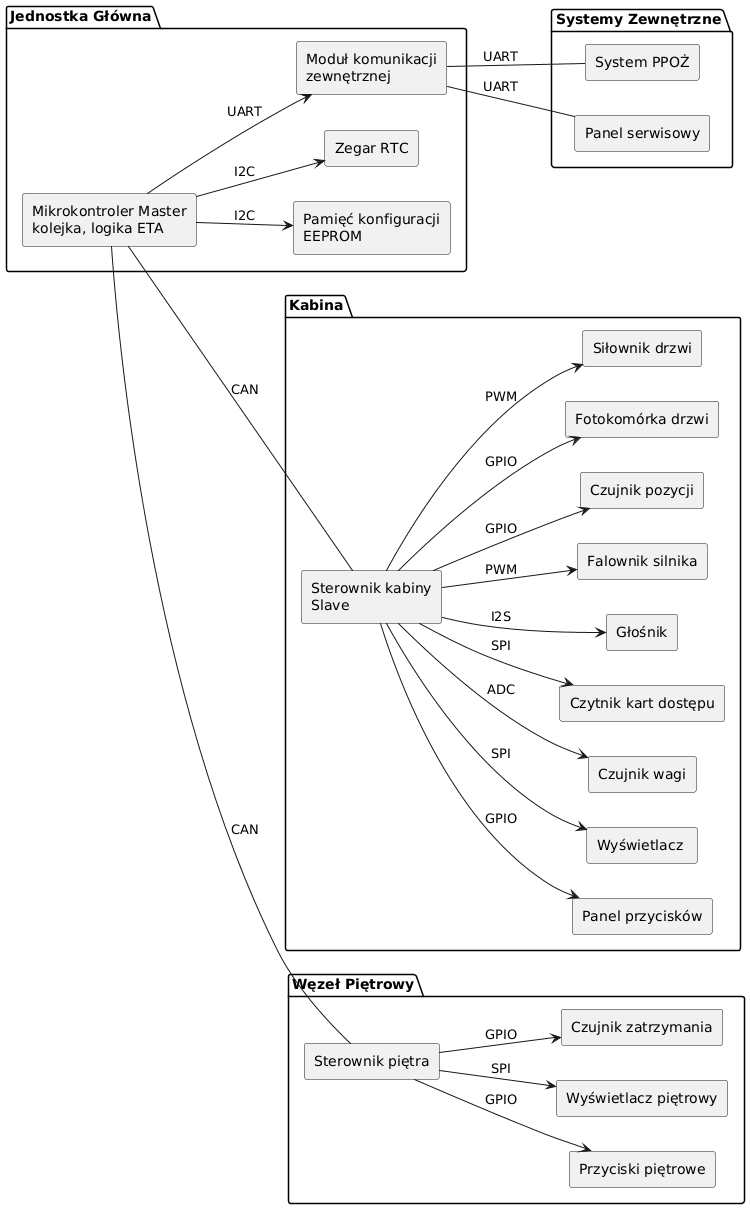
\includegraphics[height=\dimexpr\textheight-1cm\relax,keepaspectratio]{03 Diagram komponentów/Diagram.png}
\end{center}
\pagebreak
\textbf{Jednostka Główna} to węzeł nadrzędny realizujący logikę kolejkowania zadań i wyznaczania trasy kabiny. Pamięć konfiguracyjna i zegar RTC podłączone są przez I2C, moduł komunikacji zewnętrznej przez UART.

\textbf{Kabina} zawiera sterownik Slave obsługujący wszystkie podzespoły. Przyciski i czujniki binarne podłączone są przez GPIO, wyświetlacz i czytnik kart przez SPI, czujnik wagi przez ADC, głośnik przez I2S, falownik silnika i siłownik drzwi przez PWM.

\textbf{Węzeł Piętrowy} obsługuje przyciski i wyświetlacz na każdym piętrze. Komunikuje się z Jednostką Główną przez magistralę CAN, podobnie jak Kabina. CAN został wybrany ze względu na odporność na zakłócenia elektromagnetyczne panujące w szybie windy.

\textbf{Systemy Zewnętrzne} -- PPOŻ i panel serwisowy -- komunikują się przez moduł zewnętrzny oddzielony od magistrali CAN, co zapewnia niezależność systemu bezpieczeństwa.

\section{Dane w systemie}

\subsection{Pozycja kabiny}

\begin{tabularx}{\textwidth}{lX}
\toprule
\textbf{Atrybut} & \textbf{Wartość} \\
\midrule
Wielkość fizyczna & Położenie liniowe \\
Jednostka & Milimetry [mm] \\
Zakres & 0 -- maksymalna wysokość szybu \\
Rozdzielczość przechowywana & 1 mm \\
Rozdzielczość wyświetlana & Numer piętra (liczba całkowita) \\
Format wymiany & \texttt{uint32} -- surowa wartość z enkodera \\
Źródło & Czujnik pozycji \\
Odbiorcy & Master, wyświetlacz kabiny, wyświetlacz piętrowy \\
\bottomrule
\end{tabularx}

\subsection{Waga kabiny}

\begin{tabularx}{\textwidth}{lX}
\toprule
\textbf{Atrybut} & \textbf{Wartość} \\
\midrule
Wielkość fizyczna & Masa \\
Jednostka & Kilogramy [kg] \\
Zakres & 0 -- 150\% udźwigu nominalnego \\
Rozdzielczość przechowywana & 0.1 kg \\
Rozdzielczość wyświetlana & Niewyświetlana użytkownikowi \\
Format wymiany & \texttt{float32} -- odczyt ADC przeliczony na kg \\
Źródło & Czujnik wagi \\
Odbiorcy & Sterownik kabiny, Master \\
\bottomrule
\end{tabularx}

\subsection{Żądania jazdy}

\begin{tabularx}{\textwidth}{lX}
\toprule
\textbf{Atrybut} & \textbf{Wartość} \\
\midrule
Wielkość fizyczna & Brak -- dane logiczne \\
Jednostka & Brak \\
Zakres & Piętro: 0 -- N, kierunek: \{góra, dół\} \\
Rozdzielczość przechowywana & 1 piętro \\
Rozdzielczość wyświetlana & Podświetlenie przycisku wybranego piętra \\
Format wymiany & \texttt{\{floor: uint8, direction: enum, source: enum\}} \\
Źródło & Panel przycisków kabiny, przyciski piętrowe \\
Odbiorcy & Master -- kolejka zadań \\
\bottomrule
\end{tabularx}

\subsection{Stan drzwi}

\begin{tabularx}{\textwidth}{lX}
\toprule
\textbf{Atrybut} & \textbf{Wartość} \\
\midrule
Wielkość fizyczna & Brak -- dane logiczne \\
Jednostka & Brak \\
Zakres & \{otwarte, zamknięte, w ruchu, zablokowane\} \\
Rozdzielczość przechowywana & Enum 2 bity \\
Rozdzielczość wyświetlana & Niewyświetlany bezpośrednio \\
Format wymiany & \texttt{uint8} -- enum stanu \\
Źródło & Fotokomórka drzwi, siłownik drzwi \\
Odbiorcy & Sterownik kabiny, Master \\
\bottomrule
\end{tabularx}

\subsection{Prędkość kabiny}

\begin{tabularx}{\textwidth}{lX}
\toprule
\textbf{Atrybut} & \textbf{Wartość} \\
\midrule
Wielkość fizyczna & Prędkość liniowa \\
Jednostka & Milimetry na sekundę [mm/s] \\
Zakres & 0 -- 2500 mm/s \\
Rozdzielczość przechowywana & 1 mm/s \\
Rozdzielczość wyświetlana & Niewyświetlana użytkownikowi \\
Format wymiany & \texttt{uint16} \\
Źródło & Wyliczana z czujnika pozycji \\
Odbiorcy & Sterownik kabiny, falownik silnika \\
\bottomrule
\end{tabularx}

\subsection{Tryb pracy systemu}

\begin{tabularx}{\textwidth}{lX}
\toprule
\textbf{Atrybut} & \textbf{Wartość} \\
\midrule
Wielkość fizyczna & Brak -- dane logiczne \\
Jednostka & Brak \\
Zakres & \{normalny, serwisowy, awaryjny PPOŻ, przeciążenie\} \\
Rozdzielczość przechowywana & Enum 3 bity \\
Rozdzielczość wyświetlana & Komunikat na wyświetlaczu i głośniku \\
Format wymiany & \texttt{uint8} -- enum trybu \\
Źródło & Master, System PPOŻ, Panel serwisowy \\
Odbiorcy & Wszystkie komponenty systemu \\
\bottomrule
\end{tabularx}

\subsection{Parametry konfiguracyjne}

\begin{tabularx}{\textwidth}{lX}
\toprule
\textbf{Atrybut} & \textbf{Wartość} \\
\midrule
Wielkość fizyczna & Brak -- nastawy serwisowe \\
Jednostka & Zależna od parametru \\
Zakres & Czas otwarcia drzwi: 1--10 s, prędkość nominalna: 100--2500 mm/s, piętro bazowe: 0--N \\
Rozdzielczość przechowywana & Zależna od parametru \\
Rozdzielczość wyświetlana & Wartość liczbowa na panelu serwisowym \\
Format wymiany & \texttt{\{param\_id: uint8, value: uint32\}} \\
Źródło & Panel serwisowy \\
Odbiorcy & Pamięć EEPROM, Master \\
\bottomrule
\end{tabularx}

\subsection{Uprawnienia dostępu}

\begin{tabularx}{\textwidth}{lX}
\toprule
\textbf{Atrybut} & \textbf{Wartość} \\
\midrule
Wielkość fizyczna & Brak -- dane logiczne \\
Jednostka & Brak \\
Zakres & ID karty: 0 -- $2^{32}$, poziom dostępu: \{pasażer, serwis, służby\} \\
Rozdzielczość przechowywana & 32-bitowe ID karty \\
Rozdzielczość wyświetlana & Niewyświetlane \\
Format wymiany & \texttt{\{card\_id: uint32, access\_level: uint8\}} \\
Źródło & Czytnik kart dostępu \\
Odbiorcy & Master, pamięć konfiguracji \\
\bottomrule
\end{tabularx}

\subsection{Relacje między danymi}

\textbf{Żądania jazdy} trafiają do Mastera, który porównuje je z \textbf{pozycją kabiny} i generuje polecenia ruchu.

\textbf{Waga kabiny} nadpisuje żądania jazdy -- przekroczenie progu wymusza tryb przeciążenia i blokuje ruch.

\textbf{Stan drzwi} blokuje zmianę \textbf{prędkości kabiny} -- jazda możliwa tylko przy drzwiach zamkniętych i zaryglowanych.

\textbf{Tryb pracy} jest nadrzędny dla całego systemu -- tryb awaryjny PPOŻ anuluje wszystkie żądania i wymusza zjazd na piętro ewakuacyjne.

\textbf{Uprawnienia dostępu} filtrują żądania jazdy na piętra z ograniczonym dostępem.

\textbf{Parametry konfiguracyjne} z EEPROM definiują wartości graniczne dla prędkości, czasu otwarcia drzwi i piętra bazowego.
\end{document}
